\documentclass[12pt]{article}\usepackage[]{graphicx}\usepackage[]{color}
%% maxwidth is the original width if it is less than linewidth
%% otherwise use linewidth (to make sure the graphics do not exceed the margin)
\makeatletter
\def\maxwidth{ %
  \ifdim\Gin@nat@width>\linewidth
    \linewidth
  \else
    \Gin@nat@width
  \fi
}
\makeatother

\definecolor{fgcolor}{rgb}{0.345, 0.345, 0.345}
\newcommand{\hlnum}[1]{\textcolor[rgb]{0.686,0.059,0.569}{#1}}%
\newcommand{\hlstr}[1]{\textcolor[rgb]{0.192,0.494,0.8}{#1}}%
\newcommand{\hlcom}[1]{\textcolor[rgb]{0.678,0.584,0.686}{\textit{#1}}}%
\newcommand{\hlopt}[1]{\textcolor[rgb]{0,0,0}{#1}}%
\newcommand{\hlstd}[1]{\textcolor[rgb]{0.345,0.345,0.345}{#1}}%
\newcommand{\hlkwa}[1]{\textcolor[rgb]{0.161,0.373,0.58}{\textbf{#1}}}%
\newcommand{\hlkwb}[1]{\textcolor[rgb]{0.69,0.353,0.396}{#1}}%
\newcommand{\hlkwc}[1]{\textcolor[rgb]{0.333,0.667,0.333}{#1}}%
\newcommand{\hlkwd}[1]{\textcolor[rgb]{0.737,0.353,0.396}{\textbf{#1}}}%
\let\hlipl\hlkwb

\usepackage{framed}
\makeatletter
\newenvironment{kframe}{%
 \def\at@end@of@kframe{}%
 \ifinner\ifhmode%
  \def\at@end@of@kframe{\end{minipage}}%
  \begin{minipage}{\columnwidth}%
 \fi\fi%
 \def\FrameCommand##1{\hskip\@totalleftmargin \hskip-\fboxsep
 \colorbox{shadecolor}{##1}\hskip-\fboxsep
     % There is no \\@totalrightmargin, so:
     \hskip-\linewidth \hskip-\@totalleftmargin \hskip\columnwidth}%
 \MakeFramed {\advance\hsize-\width
   \@totalleftmargin\z@ \linewidth\hsize
   \@setminipage}}%
 {\par\unskip\endMakeFramed%
 \at@end@of@kframe}
\makeatother

\definecolor{shadecolor}{rgb}{.97, .97, .97}
\definecolor{messagecolor}{rgb}{0, 0, 0}
\definecolor{warningcolor}{rgb}{1, 0, 1}
\definecolor{errorcolor}{rgb}{1, 0, 0}
\newenvironment{knitrout}{}{} % an empty environment to be redefined in TeX

\usepackage{alltt}
\usepackage{amsmath}
\usepackage{mathtools}
\usepackage{amssymb}
%\usepackage{boodox-cal}
%\usepackage[margin=1in]{geometry}
\usepackage[cm]{fullpage}
\usepackage{textcomp}
\usepackage{enumitem}
\usepackage[usenames,dvipsnames,svgnames,table]{xcolor}
\usepackage{graphicx}
\usepackage{titlesec}
\usepackage[titletoc,toc,title]{appendix}
\usepackage{chngcntr}
\counterwithin{figure}{section}
\counterwithin{equation}{section}
\counterwithin{table}{section}
\DeclareGraphicsExtensions{.pdf,.png,.jpg,.jpeg}

\renewcommand{\baselinestretch}{1.25}
%\addtolength{\textheight}{3ex}
\setlength{\parindent}{0cm}
\addtolength{\parskip}{2ex}

\usepackage{hyperref}
\hypersetup{pdfborder={0 0 0}}

\newcommand{\mydef}{\stackrel{\mbox{\small def}}{=}}
\newcommand{\Sd}[1]{\mbox{Sd}(#1)}
\newcommand{\E}[1]{\mbox{E}[#1]}
\newcommand{\Var}[1]{\mbox{Var}[#1]}
\newcommand{\sign}[1]{\mbox{sign}\left(#1\right)}
\IfFileExists{upquote.sty}{\usepackage{upquote}}{}
\begin{document}
\title{
RadiusIntelligence Code Challenge\\
\author{
{Dr.~H.~Pezeshki}
}}

\maketitle
%\thispagestyle{empty}
%\newpage
\tableofcontents
\newpage





\section{Prompt}
This note has been prepared on \today\ by Dr.\ H.\ Pezeshki in response to the Radius Intelligence
coding challenge.\\~\\
The \texttt{R} statistical programming environment \cite{ritself} has been chosen, and the \texttt{knitr} package
\cite{knitr} has been used for document preparation.

\section{Input data}
The (expanded) input data is in \texttt{JSON} format. This was converted into a standard R \texttt{data.frame}
using the R \texttt{jsonlite} package \cite{jsonlite}. 
\begin{knitrout}\footnotesize
\definecolor{shadecolor}{rgb}{0.969, 0.969, 0.969}\color{fgcolor}\begin{kframe}
\begin{alltt}
\hlstd{> }\hlkwd{require} \hlstd{(jsonlite)}
\hlstd{> }\hlstd{theInput} \hlkwb{=} \hlkwd{fromJSON} \hlstd{(}\hlkwc{txt} \hlstd{=} \hlstr{'../provided/datascience-cc-1-master/data_analysis.json'}\hlstd{)}
\hlstd{> }\hlkwd{str} \hlstd{(theInput)}
\end{alltt}
\begin{verbatim}
'data.frame':	1000000 obs. of  10 variables:
 $ city            : chr  "SAN DIEGO" "ATLANTA" "NEOSHO" "CINCINNATI" ...
 $ name            : chr  "AMD CUSTOM" "Real Hope Real Estate Inc" "Jimmy Sexton Photography" "YOU'RE ART" ...
 $ zip             : chr  "92131" "30345" "64850" "45243" ...
 $ revenue         : chr  "$20 to 50 Million" "Less Than $500,000" "Less Than $500,000" "Less Than $500,000" ...
 $ time_in_business: chr  "10+ years" "10+ years" "10+ years" "10+ years" ...
 $ phone           : chr  "3123628000" NA "4046331779" "4174513798" ...
 $ state           : chr  "CA" "GA" "MO" "OH" ...
 $ address         : chr  "10085 SCRIPPS RANCH CT STE A" "2566 SHALLOWFORD RD NE STE 104 # 302" "212 E MAIN ST" "6032 CHEROKEE DR" ...
 $ headcount       : chr  "50 to 99" "1 to 4" "1 to 4" "1 to 4" ...
 $ category_code   : chr  "44420000" "31490000" "53120000" "54000000" ...
\end{verbatim}
\begin{alltt}
\hlstd{> }\hlkwd{saveRDS} \hlstd{(}\hlkwc{file}\hlstd{=}\hlstr{'theInput.rds'}\hlstd{, theInput)}
\end{alltt}
\end{kframe}
\end{knitrout}


\section{Fill rates}
The following code fragment generates the (raw) fill rates in a \texttt{data.frame} called \texttt{M}.
The results are shown in Table \ref{tbl:rawfill}.
\begin{knitrout}\footnotesize
\definecolor{shadecolor}{rgb}{0.969, 0.969, 0.969}\color{fgcolor}\begin{kframe}
\begin{alltt}
\hlstd{> }\hlstd{thefills} \hlkwb{=} \hlkwa{function} \hlstd{(}\hlkwc{x}\hlstd{) \{}
\hlstd{+ }  \hlkwd{sum} \hlstd{(}\hlkwd{is.na} \hlstd{(x))}
\hlstd{+ }\hlstd{\}}
\hlstd{> }\hlstd{tmp} \hlkwb{=} \hlkwd{apply} \hlstd{(}\hlkwc{X}\hlstd{=theInput,} \hlkwc{MARGIN} \hlstd{=} \hlnum{2}\hlstd{,} \hlkwc{FUN}\hlstd{= thefills)}
\hlstd{> }
\hlstd{> }\hlstd{Nobs} \hlkwb{=} \hlkwd{dim} \hlstd{(theInput)[}\hlnum{1}\hlstd{]}
\hlstd{> }\hlstd{vecfillrates} \hlkwb{=} \hlkwd{round} \hlstd{(}\hlnum{100} \hlopt{*} \hlstd{(Nobs} \hlopt{-} \hlstd{tmp)}\hlopt{/}\hlstd{Nobs,} \hlkwc{digits} \hlstd{=} \hlnum{3}\hlstd{)}
\hlstd{> }
\hlstd{> }\hlstd{tmp} \hlkwb{=} \hlkwd{as.numeric} \hlstd{(vecfillrates)}
\hlstd{> }\hlstd{M} \hlkwb{=} \hlkwd{as.data.frame} \hlstd{(}\hlkwc{x}\hlstd{=}\hlkwd{matrix} \hlstd{(}\hlkwc{data}\hlstd{=tmp,} \hlkwc{nrow} \hlstd{=} \hlnum{1}
\hlstd{+ }                      \hlstd{,} \hlkwc{byrow} \hlstd{=} \hlnum{TRUE}
\hlstd{+ }                      \hlstd{,} \hlkwc{dimnames} \hlstd{=} \hlkwd{list} \hlstd{(}\hlstr{'Raw fill'}\hlstd{,} \hlkwd{names} \hlstd{(vecfillrates)))}
\hlstd{+ }            \hlstd{,} \hlkwc{stringsAsFactors} \hlstd{=} \hlnum{FALSE}\hlstd{)}
\end{alltt}
\end{kframe}
\end{knitrout}
\begin{table}[htb]
\begin{center}
{\tiny

\begin{tabular}{l|r|r|r|r|r|r|r|r|r|r}
\hline
  & city & name & zip & revenue & time\_in\_business & phone & state & address & headcount & category\_code\\
\hline
Raw fill & 99.999 & 99.999 & 99.999 & 94.309 & 91.612 & 59.089 & 99.999 & 99.999 & 96.235 & 99.999\\
\hline
\end{tabular}

}
\label{tbl:rawfill}
\caption{\small Raw fill rate}
\end{center}
\end{table}

\section{True-valued fill rates}
The following code fragment was used to calculate the true fill-rates. The results are shown
in Table \ref{tbl:allfill}
\begin{knitrout}\footnotesize
\definecolor{shadecolor}{rgb}{0.969, 0.969, 0.969}\color{fgcolor}\begin{kframe}
\begin{alltt}
\hlstd{> }\hlstd{thoseMissing} \hlkwb{=} \hlkwa{function} \hlstd{(}\hlkwc{x}\hlstd{) \{}
\hlstd{+ }  \hlstd{ndx} \hlkwb{=} \hlkwd{grep} \hlstd{(}\hlkwc{pattern} \hlstd{=} \hlstr{'(^\textbackslash{}\textbackslash{}s+$|^$|null|none|^0$)'}\hlstd{,} \hlkwc{x}\hlstd{=x,} \hlkwc{ignore.case} \hlstd{=} \hlnum{TRUE}\hlstd{)}
\hlstd{+ }  \hlstd{x[ndx]} \hlkwb{=} \hlnum{NA_character_}
\hlstd{+ }  \hlstd{x}
\hlstd{+ }\hlstd{\}}
\hlstd{> }
\hlstd{> }\hlstd{hf} \hlkwb{=} \hlstd{theInput}
\hlstd{> }\hlkwa{for} \hlstd{(j} \hlkwa{in} \hlnum{1}\hlopt{:}\hlkwd{dim}\hlstd{(hf)[}\hlnum{2}\hlstd{]) \{}
\hlstd{+ }  \hlstd{hf[,j]} \hlkwb{=} \hlkwd{thoseMissing} \hlstd{(hf[,j])}
\hlstd{+ }\hlstd{\}}
\hlstd{> }
\hlstd{> }
\hlstd{> }\hlstd{tmp} \hlkwb{=} \hlkwd{apply} \hlstd{(}\hlkwc{X}\hlstd{=hf,} \hlkwc{MARGIN} \hlstd{=} \hlnum{2}\hlstd{,} \hlkwc{FUN}\hlstd{= thefills)}
\hlstd{> }
\hlstd{> }\hlstd{Nobs} \hlkwb{=} \hlkwd{dim} \hlstd{(hf)[}\hlnum{1}\hlstd{]}
\hlstd{> }\hlstd{vecTrueFillRates} \hlkwb{=} \hlkwd{round} \hlstd{(}\hlnum{100} \hlopt{*} \hlstd{(Nobs} \hlopt{-} \hlstd{tmp)}\hlopt{/}\hlstd{Nobs,} \hlkwc{digits} \hlstd{=} \hlnum{3}\hlstd{)}
\hlstd{> }\hlstd{tmp} \hlkwb{=} \hlkwd{as.numeric} \hlstd{(vecTrueFillRates)}
\hlstd{> }\hlstd{tmp} \hlkwb{=} \hlkwd{as.data.frame} \hlstd{(}\hlkwc{x}\hlstd{=}\hlkwd{matrix} \hlstd{(}\hlkwc{data}\hlstd{=tmp,} \hlkwc{nrow} \hlstd{=} \hlnum{1}
\hlstd{+ }                      \hlstd{,} \hlkwc{byrow} \hlstd{=} \hlnum{TRUE}
\hlstd{+ }                      \hlstd{,} \hlkwc{dimnames} \hlstd{=} \hlkwd{list} \hlstd{(}\hlstr{'True fill'}\hlstd{,} \hlkwd{names} \hlstd{(vecTrueFillRates)))}
\hlstd{+ }            \hlstd{,} \hlkwc{stringsAsFactors} \hlstd{=} \hlnum{FALSE}\hlstd{)}
\hlstd{> }
\hlstd{> }\hlstd{M} \hlkwb{=} \hlkwd{rbind} \hlstd{(M, tmp)}
\hlstd{> }\hlcom{# print (M)}
\end{alltt}
\end{kframe}
\end{knitrout}
\begin{table}[htb]
\begin{center}
{\tiny

\begin{tabular}{l|r|r|r|r|r|r|r|r|r|r}
\hline
  & city & name & zip & revenue & time\_in\_business & phone & state & address & headcount & category\_code\\
\hline
Raw fill & 99.999 & 99.999 & 99.999 & 94.309 & 91.612 & 59.089 & 99.999 & 99.999 & 96.235 & 99.999\\
\hline
True fill & 99.990 & 99.984 & 99.989 & 94.300 & 91.605 & 59.080 & 99.990 & 99.989 & 96.227 & 99.991\\
\hline
\end{tabular}

}
\end{center}
\label{tbl:allfill}
\caption{\small Raw and true fill rates}
\end{table}

\section{Cardinalities of individual columns}
The following code fragment was used to calculate the cardinalities displayed in Table \ref{tbl:card}
\begin{knitrout}\footnotesize
\definecolor{shadecolor}{rgb}{0.969, 0.969, 0.969}\color{fgcolor}\begin{kframe}
\begin{alltt}
\hlstd{> }\hlstd{card} \hlkwb{=} \hlkwa{function} \hlstd{(}\hlkwc{x}\hlstd{) \{}
\hlstd{+ }  \hlkwd{length} \hlstd{(}\hlkwd{unique} \hlstd{(}\hlkwd{na.omit} \hlstd{(x)))}
\hlstd{+ }\hlstd{\}}
\hlstd{> }
\hlstd{> }\hlstd{cardinalities} \hlkwb{=} \hlkwd{apply} \hlstd{(}\hlkwc{X}\hlstd{=hf,} \hlkwc{MARGIN} \hlstd{=} \hlnum{2}\hlstd{,} \hlkwc{FUN} \hlstd{= card)}
\hlstd{> }\hlstd{tmp} \hlkwb{=} \hlkwd{as.numeric} \hlstd{(cardinalities)}
\hlstd{> }\hlstd{tmp} \hlkwb{=} \hlkwd{as.data.frame} \hlstd{(}\hlkwc{x}\hlstd{=}\hlkwd{matrix} \hlstd{(}\hlkwc{data}\hlstd{=tmp,} \hlkwc{nrow} \hlstd{=} \hlnum{1}
\hlstd{+ }                      \hlstd{,} \hlkwc{byrow} \hlstd{=} \hlnum{TRUE}
\hlstd{+ }                      \hlstd{,} \hlkwc{dimnames} \hlstd{=} \hlkwd{list} \hlstd{(}\hlstr{'Cardinalities'}\hlstd{,} \hlkwd{names} \hlstd{(vecTrueFillRates)))}
\hlstd{+ }            \hlstd{,} \hlkwc{stringsAsFactors} \hlstd{=} \hlnum{FALSE}\hlstd{)}
\end{alltt}
\end{kframe}
\end{knitrout}
\begin{table}[htb]
\begin{center}
{\tiny

\begin{tabular}{l|r|r|r|r|r|r|r|r|r|r}
\hline
  & city & name & zip & revenue & time\_in\_business & phone & state & address & headcount & category\_code\\
\hline
Cardinalities & 13714 & 890653 & 26391 & 11 & 5 & 575148 & 53 & 892103 & 9 & 1178\\
\hline
\end{tabular}

}
\end{center}
\label{tbl:card}
\caption{\small cardinalities}
\end{table}

\section{Exploratory analysis}
One clearly observes that the columns \texttt{revenue}, \texttt{time\_in\_business} and \texttt{headcount}
are \textit{ordered factors}, and a measure of quantitative analysis is possible if one uses \textit{ranks}
of the entries rather than factor level numbers. Thus, we first convert these fields from \texttt{character}
to \texttt{ordered factor} as follows:
\begin{knitrout}\footnotesize
\definecolor{shadecolor}{rgb}{0.969, 0.969, 0.969}\color{fgcolor}\begin{kframe}
\begin{alltt}
\hlstd{> }\hlstd{hc_levels} \hlkwb{=} \hlkwd{c}\hlstd{(}
\hlstd{+ }  \hlstr{"1 to 4"}\hlstd{,} \hlstr{"5 to 9"}\hlstd{,} \hlstr{"10 to 19"}\hlstd{,} \hlstr{"20 to 49"}\hlstd{,} \hlstr{"50 to 99"}
\hlstd{+ }  \hlstd{,} \hlstr{"100 to 249"}\hlstd{,} \hlstr{"250 to 499"}\hlstd{,} \hlstr{"500 to 999"}\hlstd{,} \hlstr{"Over 1,000"}
\hlstd{+ }\hlstd{)}
\hlstd{> }\hlstd{hf}\hlopt{$}\hlstd{headcount} \hlkwb{=} \hlkwd{factor} \hlstd{(}\hlkwc{x}\hlstd{=hf}\hlopt{$}\hlstd{headcount,} \hlkwc{levels} \hlstd{= hc_levels,} \hlkwc{ordered} \hlstd{=} \hlnum{TRUE}\hlstd{)}
\hlstd{> }
\hlstd{> }\hlstd{revenue_levels} \hlkwb{=} \hlkwd{c} \hlstd{(}
\hlstd{+ }  \hlstr{"Less Than $500,000"}\hlstd{,} \hlstr{"$500,000 to $1 Million"}\hlstd{,} \hlstr{"$1 to 2.5 Million"}\hlstd{,} \hlstr{"$2.5 to 5 Million"}
\hlstd{+ }  \hlstd{,} \hlstr{"$5 to 10 Million"}\hlstd{,} \hlstr{"$10 to 20 Million"}\hlstd{,} \hlstr{"$20 to 50 Million"}
\hlstd{+ }  \hlstd{,} \hlstr{"$50 to 100 Million"}\hlstd{,} \hlstr{"$100 to 500 Million"}\hlstd{,} \hlstr{"Over $500 Million"}\hlstd{,} \hlstr{"Over $1 Billion"}
\hlstd{+ }\hlstd{)}
\hlstd{> }\hlstd{hf}\hlopt{$}\hlstd{revenue} \hlkwb{=} \hlkwd{factor} \hlstd{(}\hlkwc{x} \hlstd{= hf}\hlopt{$}\hlstd{revenue,} \hlkwc{levels} \hlstd{= revenue_levels,} \hlkwc{ordered} \hlstd{=} \hlnum{TRUE}\hlstd{)}
\hlstd{> }
\hlstd{> }\hlstd{time_in_business_levels} \hlkwb{=} \hlkwd{c}\hlstd{(}
\hlstd{+ }  \hlstr{"Less than a year"}\hlstd{,} \hlstr{"1-2 years"}\hlstd{,} \hlstr{"3-5 years"}\hlstd{,} \hlstr{"6-10 years"}\hlstd{,} \hlstr{"10+ years"}
\hlstd{+ }\hlstd{)}
\hlstd{> }\hlstd{hf}\hlopt{$}\hlstd{time_in_business} \hlkwb{=} \hlkwd{factor} \hlstd{(}\hlkwc{x} \hlstd{= hf}\hlopt{$}\hlstd{time_in_business,} \hlkwc{levels} \hlstd{= time_in_business_levels,} \hlkwc{ordered} \hlstd{=} \hlnum{TRUE}\hlstd{)}
\hlstd{> }\hlkwd{str} \hlstd{(hf)}
\end{alltt}
\begin{verbatim}
'data.frame':	1000000 obs. of  10 variables:
 $ city            : chr  "SAN DIEGO" "ATLANTA" "NEOSHO" "CINCINNATI" ...
 $ name            : chr  "AMD CUSTOM" "Real Hope Real Estate Inc" "Jimmy Sexton Photography" "YOU'RE ART" ...
 $ zip             : chr  "92131" "30345" "64850" "45243" ...
 $ revenue         : Ord.factor w/ 11 levels "Less Than $500,000"<..: 7 1 1 1 2 4 3 1 1 1 ...
 $ time_in_business: Ord.factor w/ 5 levels "Less than a year"<..: 5 5 5 5 5 4 5 5 5 NA ...
 $ phone           : chr  "3123628000" NA "4046331779" "4174513798" ...
 $ state           : chr  "CA" "GA" "MO" "OH" ...
 $ address         : chr  "10085 SCRIPPS RANCH CT STE A" "2566 SHALLOWFORD RD NE STE 104 # 302" "212 E MAIN ST" "6032 CHEROKEE DR" ...
 $ headcount       : Ord.factor w/ 9 levels "1 to 4"<"5 to 9"<..: 5 1 1 1 1 2 1 1 1 3 ...
 $ category_code   : chr  "44420000" "31490000" "53120000" "54000000" ...
\end{verbatim}
\end{kframe}
\end{knitrout}
Let us inquire if time-in-business, revenue and headcount are predictive of one another. We can
quantify this using the \textit{rank correlations} of the three columns.
The following code fragment was used to generate the result in Figure \ref{fig:rankcor}.
One observes that there is no observable correlation amongst these three covariates and any predictive analysis of
a new feature of the business (besides the ones in the input data) should use all three of headcount, revenue
and time-in-business.
\begin{knitrout}\footnotesize
\definecolor{shadecolor}{rgb}{0.969, 0.969, 0.969}\color{fgcolor}\begin{kframe}
\begin{alltt}
\hlstd{> }\hlstd{tmp} \hlkwb{=} \hlstd{hf[,} \hlkwd{c}\hlstd{(}\hlstr{'time_in_business'}\hlstd{,} \hlstr{'revenue'}\hlstd{,} \hlstr{'headcount'}\hlstd{)]}
\hlstd{> }\hlstd{tmp}\hlopt{$}\hlstd{time_in_business} \hlkwb{=} \hlkwd{as.numeric} \hlstd{(tmp}\hlopt{$}\hlstd{time_in_business)}
\hlstd{> }\hlstd{tmp}\hlopt{$}\hlstd{revenue} \hlkwb{=} \hlkwd{as.numeric} \hlstd{(tmp}\hlopt{$}\hlstd{revenue)}
\hlstd{> }\hlstd{tmp}\hlopt{$}\hlstd{headcount} \hlkwb{=} \hlkwd{as.numeric} \hlstd{(tmp}\hlopt{$}\hlstd{headcount)}
\hlstd{> }\hlstd{theCorrelations} \hlkwb{=} \hlkwd{cor} \hlstd{(tmp,} \hlkwc{use}\hlstd{=}\hlstr{"pairwise.complete.obs"}\hlstd{,} \hlkwc{method} \hlstd{=} \hlstr{"spearman"}\hlstd{)}
\end{alltt}
\end{kframe}
\end{knitrout}

\begin{figure}[htb]
\begin{center}
\begin{knitrout}\footnotesize
\definecolor{shadecolor}{rgb}{0.969, 0.969, 0.969}\color{fgcolor}
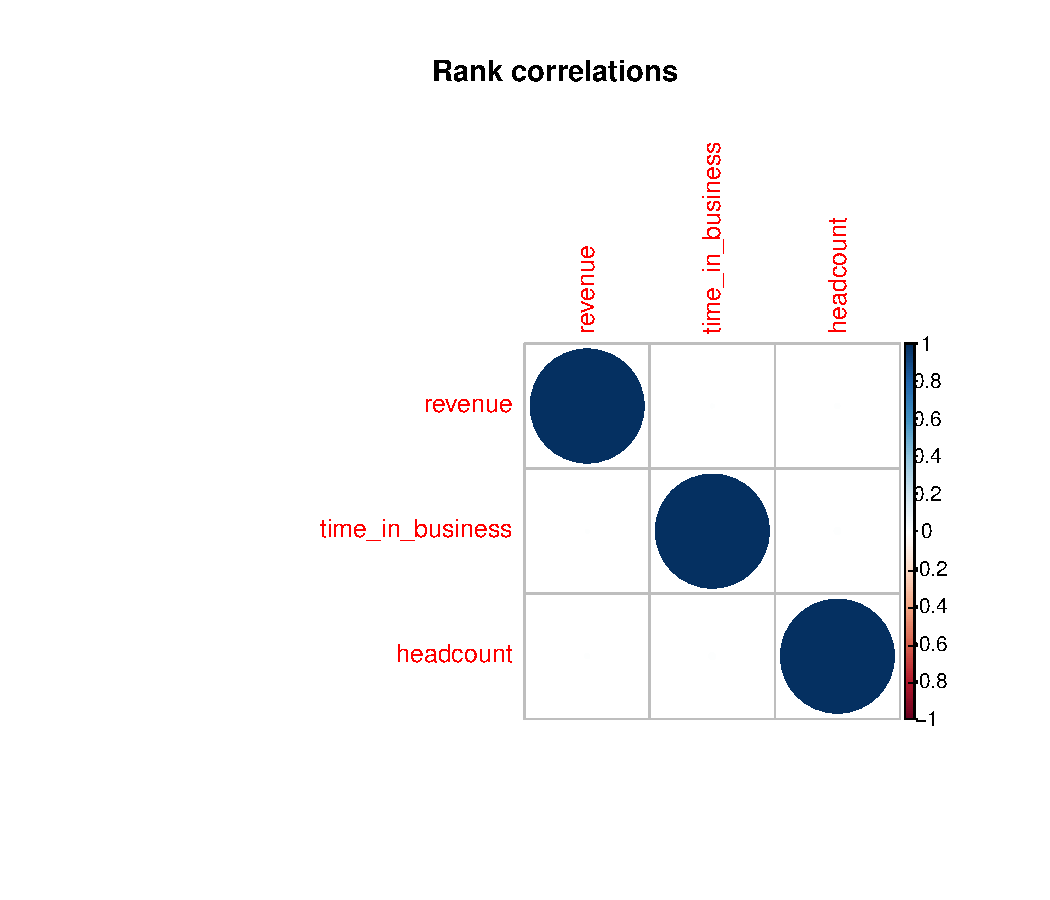
\includegraphics[width=\maxwidth]{figure/unnamed-chunk-8-1} 

\end{knitrout}
\caption{\small Rank correlations}\label{fig:rankcor}
\end{center}
\end{figure}

\clearpage
\bibliographystyle{plain}
\bibliography{mybib}
\end{document}
